\documentclass[11pt]{article}

\usepackage[a4paper,margin=1in]{geometry}
\usepackage{amsmath}
\usepackage{amssymb}
\usepackage{booktabs}
\usepackage{tabularx}
\usepackage{float}
\usepackage{graphicx}
\usepackage[hidelinks]{hyperref}
\usepackage[authoryear,round]{natbib}
\usepackage{siunitx}
\usepackage{tikz}
\usetikzlibrary{arrows.meta,positioning}
\sisetup{group-separator={,}, group-minimum-digits=4}

\title{Diversity at Fixed Support:\\
A Follow-Up Experiment on the Unmanipulated Signal}
\author{Yannik Queisler}
\date{\today}

\begin{document}
\maketitle

\begin{abstract}
\noindent The patch benchmark treated representational diversity as one of five signals a mitigation method might read, but never varied it. Every condition changed diversity only as a side effect of changing patch counts, so the diversity shortage and the nominal shortage moved together and the one diversity-reading method was judged on conditions that contained no isolated diversity shortage. This protocol closes that gap with a deliberately small experiment. Starting from the benchmark's frozen balanced and severe training manifests, it preserves every count those manifests fix---the per-class patch totals, the case set, and the number of patches each case contributes---and re-selects only which patches occupy those slots, using three deterministic rules over frozen Virchow2 features: patches nearest the class-and-case centroid, the benchmark's uniform draw, and a farthest-point spread. Prevalence, nominal support, independent support, and the frozen support--difficulty alignment are therefore identical across the three levels by construction, and within-class feature volume is the only quantity that moves. Crossing the three levels with two allocations on BRACS and TCGA-UT gives twelve training sets per split and asks three questions: whether a diversity shortage damages discrimination or probability quality at all, whether that damage is larger under a long-tailed allocation, and whether a diversity-reading class weight repairs it better than a prevalence-reading one. A manipulation gate precedes all three, so a null result can be attributed to the signal rather than to a construction that failed to move it.
\end{abstract}

\setcounter{tocdepth}{2}
\tableofcontents
\clearpage

\section{Motivation}
\label{sec:motivation}
A class can be underserved for several distinct reasons, and the count that marks it as rare does not say which. The signal taxonomy behind this line of work names five candidates: class prevalence, nominal example support, independent patient or slide support, class difficulty, and representational diversity---how much variation a class spans under the available feature representation \citep{queisler2026imbalanceMethods}. A mitigation method reads one of these signals to decide where to intervene, so the practical question is not only whether a method helps but whether the signal it reads is the one that is actually short.

The patch benchmark answered that question for four of the five signals and left the fifth open \citep{queisler2026benchmarkProtocol,queisler2026benchmarkResults}. Its controlled conditions manipulated two things: how a fixed patch budget was allocated among classes, and how many patients supplied an identical allocation. Class difficulty entered through a third, non-manipulated axis, the assignment that decides which classes receive the scarce allocation. Representational diversity entered only as a realized description. Because diversity was reduced solely by removing patches, the realized diversity shortage moved with the nominal shortage under every condition, and the benchmark states the consequence plainly: no condition creates a diversity shortage while holding patch counts fixed, and the diversity axis was never manipulated.

Three costs follow from that omission. First, it is unknown whether a diversity shortage causes any damage on its own; the benchmark's exploratory association model returned a diversity coefficient whose sign was the reverse of the expected direction, and the results report warns against reading it causally precisely because the predictor was collinear with the manipulation. Second, the single diversity-reading method in the roster, semantic-scale weighted cross-entropy, was evaluated only on conditions dominated by a nominal shortage. Losing there says that its weight map is a poor substitute for a prevalence weight under patch deprivation; it says nothing about whether reading diversity helps when diversity is what is missing. Third, and most consequential for the overarching goal of designing a mitigation method for long-tailed histopathology, there is currently no evidence on which to decide whether such a method should carry a diversity term at all.

This report specifies a follow-up experiment that supplies that evidence. It is deliberately narrow. One factor is added, two allocations are retained, three method arms are kept, and every other design element---partitions, features, model family, endpoints, and gate discipline---is inherited unchanged from the benchmark so that the new numbers are directly comparable with the existing ones.

\section{Research Questions}
\label{sec:rqs}
The experiment manipulates within-class representational diversity while holding every count fixed, and asks:
\begin{description}
  \item[RQ-D1 (damage).] At fixed prevalence, nominal patch support, and independent patient support, does reducing within-class representational diversity degrade tail discrimination or probability quality?
  \item[RQ-D2 (interaction).] Is any such degradation larger under a severely long-tailed allocation than under a balanced one---that is, does a diversity shortage compound a nominal shortage?
  \item[RQ-D3 (mitigation).] Where RQ-D1 establishes a material deficit, does a class weight that reads diversity recover more of it than a class weight that reads prevalence?
\end{description}
\noindent The three questions are ordered as a chain. RQ-D3 is interpreted only where RQ-D1's deficit gate opens, mirroring the benchmark's rule that recovery is meaningless without an established deficit. RQ-D2 is the question that connects the experiment to long-tailed learning: a diversity shortage that matters only under balance would be a curiosity, whereas one that compounds under a long tail is a design requirement for a mitigation method.

Preceding all three is a manipulation check, described in Section~\ref{sec:manipulation}. Because the whole design rests on moving one signal while pinning the others, a construction that fails to move it must be reported as a failed manipulation rather than a null effect.

\section{Design}
\label{sec:design}
The design reuses the benchmark's frozen training manifests as fixed scaffolding and changes only the identity of the patches that fill them. This section states what is held fixed, defines the three selection rules that vary, and gives the resulting grid.

\subsection{What is held fixed and what varies}
\label{sec:fixed-varied}
Two allocations are inherited from the benchmark: the size-matched \emph{balanced} allocation, in which a shared training total is divided evenly among classes, and the \emph{severe} allocation, in which the same total is redistributed so that the largest class holds about one hundred times as many patches as the smallest. Both draw from the benchmark's concentrated patient pool. Each frozen manifest fixes, for every class $c$ and every contributing case $g$, a patch count $n_{cg}$; summing over cases gives the class total $N_c$, and the set of cases with $n_{cg}>0$ gives the class's independent support.

The manipulation preserves all of these quantities exactly. For each $(c,g)$ pair, the same number $n_{cg}$ of patches is drawn, from the same eligible pool, under a different selection rule. The consequence is that class shares, the imbalance ratio, the nominal support of every class, the number of contributing patients per class, and the frozen pilot difficulty---and therefore the support--difficulty alignment---are numerically identical across the three levels. Table~\ref{tab:fixed-varied} states this explicitly, and Figure~\ref{fig:construction} places it in the construction sequence.

\begin{table}[H]
  \centering
  \small
  \begin{tabularx}{\linewidth}{@{}l>{\raggedright\arraybackslash}X@{}}
    \toprule
    Quantity & Status across the three diversity levels \\
    \midrule
    Class shares and imbalance ratio $\rho$ & Fixed by the inherited manifest \\
    Per-class patch total $N_c$ & Fixed \\
    Per-case patch count $n_{cg}$ and case set & Fixed, pair by pair \\
    Frozen pilot difficulty and alignment $A$ & Fixed; estimated before conditions exist \\
    Validation and test cohorts & Fixed at their natural class distributions \\
    Feature extractor, model family, update policy & Fixed \\
    \midrule
    Which patches occupy the fixed slots & \textbf{Varied} by the selection rule \\
    Within-class feature volume $S'_c$ & \textbf{Varies as a consequence} \\
    \bottomrule
  \end{tabularx}
  \caption{The manipulation changes patch identity only. Because prevalence, nominal support, and independent support are pinned pair by pair rather than merely in aggregate, they cannot drift with the diversity level, which is the decoupling the benchmark's allocation-based conditions could not achieve.}
  \label{tab:fixed-varied}
\end{table}

\begin{figure}[H]
  \centering
  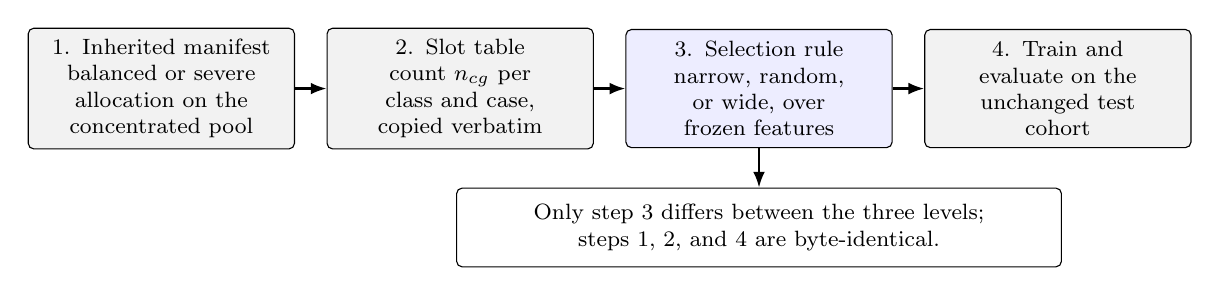
\begin{tikzpicture}[
    box/.style={draw, rounded corners=2pt, align=center, inner sep=4pt, font=\footnotesize, text width=3.1cm, minimum height=1.5cm},
    fixed/.style={box, fill=gray!10},
    varied/.style={box, fill=blue!7},
    note/.style={draw, rounded corners=2pt, align=center, inner sep=4pt, font=\footnotesize, fill=white, text width=7.4cm, minimum height=1.0cm},
    arrow/.style={-{Latex[length=2mm]}, thick}
  ]
    \node[fixed] (manifest) {1. Inherited manifest\\balanced or severe\\allocation on the\\concentrated pool};
    \node[fixed, right=0.4cm of manifest] (slots) {2. Slot table\\count $n_{cg}$ per\\class and case,\\copied verbatim};
    \node[varied, right=0.4cm of slots] (select) {3. Selection rule\\narrow, random,\\or wide, over\\frozen features};
    \node[fixed, right=0.4cm of select] (train) {4. Train and\\evaluate on the\\unchanged test\\cohort};
    \node[note, below=0.5cm of select] (caption) {Only step 3 differs between the three levels;\\steps 1, 2, and 4 are byte-identical.};
    \draw[arrow] (manifest) -- (slots);
    \draw[arrow] (slots) -- (select);
    \draw[arrow] (select) -- (train);
    \draw[arrow] (select.south) -- (caption.north);
  \end{tikzpicture}
  \caption{Construction of one training set. The inherited manifest supplies the counts; the selection rule supplies the patches. Holding step~2 fixed pair by pair is what separates the diversity signal from the support signals.}
  \label{fig:construction}
\end{figure}

\subsection{The three selection rules}
\label{sec:rules}
Let $Z_{cg}$ be the frozen Virchow2 feature vectors of the eligible patches of class $c$ in case $g$ \citep{zimmermann2024virchow2}, and let $\mu_{cg}$ be their mean. Each rule returns exactly $n_{cg}$ of them and is deterministic given the manifest and a seed:
\begin{description}
  \item[Narrow.] The $n_{cg}$ patches with smallest Euclidean distance to $\mu_{cg}$. This concentrates the draw in the densest region of the class's appearance within that case and deliberately discards its unusual patches.
  \item[Random.] The benchmark's seeded uniform draw, retained unchanged. This level reproduces the benchmark's own training sets and serves as the anchor that ties the new numbers to the existing ones.
  \item[Wide.] Greedy farthest-point sampling, seeded at the patch closest to $\mu_{cg}$ and thereafter adding the eligible patch whose minimum distance to the already-selected set is largest. This spreads the draw across the case's appearance range.
\end{description}
\noindent Farthest-point sampling is preferred over a clustering-based spread because it needs no cluster count, is deterministic, and maximizes coverage directly rather than through a proxy. Both extreme rules operate within a case rather than across cases, which is what keeps the number of contributing patients identical; the price is that the achievable diversity contrast is bounded by within-case appearance variation. Section~\ref{sec:manipulation} makes that price measurable rather than assumed.

\subsection{Grid, arms, and budget}
\label{sec:grid}
Crossing two allocations with three selection rules gives the six training sets of Table~\ref{tab:grid}, per dataset and per split.

\begin{table}[H]
  \centering
  \small
  \begin{tabular}{@{}llll@{}}
    \toprule
    & Narrow & Random (anchor) & Wide \\
    \midrule
    Balanced allocation & \texttt{bal-narrow} & \texttt{bal-random} & \texttt{bal-wide} \\
    Severe allocation & \texttt{sev-narrow} & \texttt{sev-random} & \texttt{sev-wide} \\
    \bottomrule
  \end{tabular}
  \caption{The six training sets. Within a row, all counts are identical and only patch identity differs; between rows, the counts differ exactly as in the benchmark. The \texttt{random} column reproduces the benchmark's native-assignment conditions.}
  \label{tab:grid}
\end{table}

\noindent Two datasets carry the design: BRACS, with seven breast carcinoma subtypes annotated at region level \citep{brancati2022bracs}, and TCGA-UT, with thirty retained cancer types \citep{komura2022universalEncoding}. Both are the datasets the benchmark's results report already covers, so their partitions, class tiers, materiality thresholds, and tuned hyperparameters transfer directly, and neither requires new data preparation \citep{queisler2026datasets}. They also bracket the regime of interest: BRACS is a small multiclass problem with few cases, TCGA-UT a thirty-class problem with a pronounced natural tail. Two datasets are the replication unit; the three partitions within a dataset are repeated partitions of one cohort and are not independent replications.

Three method arms are used, chosen so that each answers one question and no more:

\begin{table}[H]
  \centering
  \small
  \begin{tabularx}{\linewidth}{@{}lll>{\raggedright\arraybackslash}X@{}}
    \toprule
    Arm & Signal read & Role & Purpose \\
    \midrule
    Cross-entropy & none & baseline & Measures the damage a diversity shortage does \\
    Semantic-scale weighted CE & diversity & matched & Reads the signal the manipulation moves \\
    Weighted CE & prevalence & unmatched & Reads a signal the manipulation holds constant \\
    \bottomrule
  \end{tabularx}
  \caption{The three arms. Both weighted arms apply a mean-one class weight to unmodified cross-entropy, so a difference between them is attributable to the signal rather than to the intervention mechanism.}
  \label{tab:arms}
\end{table}

\noindent The unmatched arm is the informative control. Its weights depend on class counts, which the manipulation pins, so its weights are numerically identical in the narrow, random, and wide cells of a given allocation. Any difference in its performance across those cells therefore reflects the training data alone, and it provides a reference against which the matched arm's ability to respond to the shortage can be judged. The matched arm, by contrast, re-estimates its signal from the current representation during training, so its weights do change with the selection rule.

The full grid is $2$ datasets $\times\ 3$ splits $\times\ 6$ training sets $\times\ 3$ arms $\times\ 5$ initialization seeds, or \num{540} classifier-head fits on cached features. The \num{180} fits in the \texttt{random} column duplicate the benchmark's native-assignment runs and are reused where the manifest provenance hash matches, leaving about \num{360} new fits. Because the feature extractor is frozen and only a small head is trained, this is a minor computation, which is the point: the experiment is small enough to run and small enough to interpret.

Hyperparameters are inherited rather than re-tuned. Each arm reuses the selection its tuning locked for the corresponding allocation in the benchmark, and the narrow and wide cells inherit the random cell's selection. Since the model family, class counts, and training budget are unchanged and only patch identity differs, the inherited settings remain admissible; Section~\ref{sec:scope} records the residual risk this carries.

\section{Manipulation Check}
\label{sec:manipulation}
The entire design depends on the selection rules actually moving within-class feature volume, so that quantity is measured before any outcome is examined. Diversity is measured exactly as in the benchmark, using the regularized log-volume that semantic-scale balanced learning defines \citep{ma2023semanticScale}. For a class $c$ with $M$ centred frozen feature vectors collected in $Z_c \in \mathbb{R}^{d\times M}$, and with pooled isotropic scaling fixing $\varepsilon=1$,
\begin{equation}
  S'_c=\tfrac{1}{2}\log_2\det\!\left(I+\frac{d}{M\varepsilon^{2}}Z_cZ_c^{\top}\right).
  \label{eq:semantic-volume}
\end{equation}
\noindent The estimate is taken on a deterministic draw with equal cases and patches per class, so it describes the shape of a class's feature cloud rather than its size. Taking the wide cell as the reference and the narrow cell as the deprived condition, the induced diversity shortage of an allocation $a$ is
\begin{equation}
  S_{\mathrm{div}}(a)=\frac{1}{K}\sum_{c=1}^{K}
  \log\frac{\max\!\big(S_c^{\prime}(\text{wide},a),\,\varepsilon_S\big)}
           {\max\!\big(S_c^{\prime}(\text{narrow},a),\,\varepsilon_S\big)},
  \qquad \varepsilon_S=\num{e-3},
  \label{eq:diversity-shortage}
\end{equation}
\noindent with the mean taken over all $K$ classes because every class is manipulated. Positive values mean the narrow cell occupies less feature volume. The companion quantities $S_{\mathrm{nom}}$ and $S_{\mathrm{ind}}$ are computed on the same cells and are expected to be exactly zero; reporting them is the audit that the construction did what it claims.

Two prespecified checks govern interpretation. The first is a headroom diagnostic: for each class and case, the ratio $h_{cg}$ of eligible pool size to drawn count $n_{cg}$ bounds how much freedom either extreme rule has, since $h_{cg}=1$ leaves none. The distribution of $h_{cg}$ is reported per dataset and allocation, separately for the tail classes, which are the classes most likely to exhaust their pool under the balanced allocation. The second is the manipulation gate: $S_{\mathrm{div}}(a)$ must exceed the largest diversity shortage the benchmark's own four comparisons realized on that dataset. Clearing this threshold establishes that the experiment induces a diversity shortage at least as large as the ones the benchmark observed, but induces it without touching any count.

If the gate does not open, the outcome is reported as a failed manipulation and no claim about the diversity signal is made. One fallback is specified in advance for that case: relax the pinning from per-case counts to per-class counts, matching only the number of contributing cases rather than each case's contribution, and selecting across the class's whole pool. This buys a larger achievable contrast at the cost of a weaker independent-support control, and it therefore requires reporting the achieved per-class patient counts alongside every result. The fallback is a documented contingency, not a second analysis to be run alongside the first.

\section{Endpoints, Estimands, and Gates}
\label{sec:endpoints}
The endpoints are those of the benchmark, unchanged, so that effect sizes can be read against the allocation-induced effects already reported. Discrimination is measured by balanced accuracy, equal to macro recall, under the case-macro estimator that aggregates within a partitioning unit first so that heavily tiled cases cannot dominate. Probability quality is measured by tail-group macro negative log likelihood in nats, where the tail group is the lowest third of classes by allocated support. Because the balanced allocation gives every class the same support and therefore no support ranking, the tail group is fixed once, from the severe allocation, and the same class set is used in both allocations; without this the two rows of Table~\ref{tab:grid} would report the same name for different class sets.

Temperature scaling is applied as a pre-committed diagnostic, not as a decision rule \citep{guo2017calibration}. The benchmark found that most of its apparent probability-quality effects dissolved once a single temperature was fitted, which means an unscaled improvement can reflect nothing more than a systematic confidence offset. Committing to the scaled endpoint in advance prevents that ambiguity from being resolved after the fact.

Three estimands follow from the three questions. Writing $M(\cdot)$ for an endpoint evaluated on the held-out cohort, the diversity damage under allocation $a$ is the contrast between the two extreme rules,
\begin{equation}
  D_{\mathrm{div}}(a)=M(\text{wide},a)-M(\text{narrow},a),
  \label{eq:damage}
\end{equation}
\noindent evaluated on the cross-entropy arm. The interaction that answers RQ-D2 is the difference of these two contrasts, $D_{\mathrm{div}}(\text{severe})-D_{\mathrm{div}}(\text{balanced})$. Recovery, defined only where the deficit gate opens, is the share of the damage a method returns,
\begin{equation}
  R(\text{method},a)=\frac{M(\text{method},\text{narrow},a)-M(\text{ce},\text{narrow},a)}{D_{\mathrm{div}}(a)}.
  \label{eq:recovery}
\end{equation}

\noindent The deficit gate follows the benchmark's two-part rule. A deficit is material when its magnitude reaches the dataset-specific minimum---$\max(\num{1}\text{ percentage point},\,2\sigma_{\mathrm{seed}})$ for balanced accuracy, and the corresponding nats threshold for tail-group macro NLL---and when its paired \num{95}\% interval excludes zero. The seed dispersion $\sigma_{\mathrm{seed}}$ is recomputed on this experiment's own \texttt{random} baseline cells using the benchmark's procedure rather than copied, because a threshold derived from different training sets would not describe this experiment's noise floor. RQ-D3 is evaluated only in cells where this gate opens.

\section{Analysis}
\label{sec:analysis}
Uncertainty and testing reuse the benchmark's machinery, which keeps the two sets of results on one scale. Intervals come from a case-block bootstrap that resamples partitioning units, so uncertainty reflects the clustering of patches within patients rather than treating patches as independent. Tests are paired permutation tests over the same blocks, comparing conditions that share held-out cases and seeds. Results from the three partitions are combined with equal weight, as in the benchmark, and are presented as repeated views of one cohort rather than as independent replications.

The confirmatory family is small enough to enumerate. Within each dataset it contains four damage tests---two allocations crossed with two endpoints---two interaction tests, one per endpoint, and the matched-versus-unmatched method contrast for each cell and endpoint where the deficit gate opens. Holm adjustment controls the family-wise error across this set jointly, per dataset. Every other comparison, including per-class breakdowns, the scaled-endpoint contrasts, and any descriptive comparison against the benchmark's own conditions, is exploratory and reported with intervals but without adjusted tests.

The report of results should lead with the manipulation check, since it conditions everything after it, then give the damage contrasts with the deficit gate outcomes, then the interaction, and only then the method contrasts in the cells that qualify. Cells whose gate does not open are recorded as not tested rather than as null results, because a method contrast computed against an immaterial deficit has an unstable denominator in Equation~\eqref{eq:recovery}.

\section{Scope and Threats to Validity}
\label{sec:scope}
Five limitations bound what this experiment can establish, and each is a consequence of a deliberate choice to keep it small.

Diversity is defined here as feature-space volume under one frozen representation. It is a measurable proxy for morphological variety, not the thing itself: two selections with equal Virchow2 volume could differ in ways a pathologist would consider important, and a different encoder could order the same selections differently. Claims are therefore about diversity as this representation measures it, which is also the definition the diversity-reading method itself uses, so the method and the manipulation at least agree on the quantity in question.

The within-case restriction bounds the achievable contrast. Pinning each case's contribution is what makes independent support incorruptible, but it also confines the manipulation to variation that exists inside a single case, which is likely smaller than variation across cases. This is the reason the manipulation gate exists, and the reason the fallback in Section~\ref{sec:manipulation} is specified in advance rather than improvised.

Hyperparameters are inherited, so a selection tuned on the random cell might suit the narrow or wide cell less well. The risk is not symmetric across arms: the matched arm re-estimates its signal during training and so adapts to the cell, whereas a fixed learning rate or weight decay does not. If the matched arm underperforms, inherited tuning is a live alternative explanation and should be stated as such rather than dismissed.

The assignment axis is dropped. The benchmark ran three tail assignments; this experiment uses the native assignment only, which removes two thirds of the conditions and is the single largest reason it stays small. The consequence is that no interaction between diversity and support--difficulty alignment can be examined here.

Finally, two datasets provide the only replication. A result that holds on BRACS and TCGA-UT is more credible than one that holds on either alone, but two datasets do not establish that a coefficient transports to a new cohort, and neither dataset was chosen at random from the space of histopathology tasks.

It is worth stating what a null result would and would not license. If the manipulation gate opens and no damage contrast reaches materiality on either dataset, the reasonable reading is that within-case representational diversity, at the magnitudes this construction can induce, is not a limiting factor for these tasks---and therefore that a mitigation method aimed at long-tailed histopathology has no evidential reason to carry a diversity term. That is a useful negative result, and it is the outcome this design is built to be able to state. It would not license the stronger claim that diversity never matters, since a construction reaching across cases, or a different representation, could induce shortages this one cannot.

\section{Summary}
\label{sec:summary}
The patch benchmark left one of its five signals unmanipulated, and in doing so left open both whether a diversity shortage damages anything and whether a diversity-reading method is worth building. This protocol specifies the smallest experiment that can close that gap: reuse the benchmark's frozen manifests, preserve every count they fix pair by pair, and vary only which patches fill the fixed slots, using a centroid-nearest rule, the original uniform draw, and a farthest-point spread. Crossing three such levels with the balanced and severe allocations on BRACS and TCGA-UT, with three method arms and the benchmark's own endpoints, gates, and inference, yields a design that isolates diversity from every count it was previously confounded with. A manipulation gate placed before the outcome analysis makes the eventual answer interpretable in either direction, which is what a signal that has never been varied requires.

\bibliographystyle{plainnat}
\bibliography{references}

\end{document}
